\documentclass{article}
\usepackage{graphicx} %package to manage images
\graphicspath{{images/}}
\usepackage{hyperref}
\usepackage{amsmath}

\usepackage[utf8x]{inputenc}
\usepackage[T1]{fontenc}
\usepackage[frenchb]{babel}
\usepackage{float}
\usepackage{listings}

% for tables
\usepackage{booktabs}
\usepackage{multirow}

% dendogram
\usepackage{tikz}

% for caption
\usepackage{caption}
\usepackage[justification=centering]{caption}

\begin{document}

\title{Introduction à la vision par ordinateur \\
TP3: Extraction de caractéristiques \\et mise
en correspondance}
\author{Thibault Kaspi - thibault.kaspi@student.ecp.fr}
\maketitle

\begin{abstract}
Présentation d'implémentations de différentes méthodes de mise en correspondance des images à l’aide de leurs points d’intérêts respectifs. Le code a été réalisé avec l'aide de deux autres étudiants: Romain Catajar et Léo Hoummady.
\end{abstract}

\section{Mise en correspondance d'images}

\begin{enumerate}
    \item \textit{Sur deux images d’une même scène, calculer les points d’intérêts. Documentez vous sur ces différentes fonctions et utilisez l’une d’entre elles pour calculer des points d’intérêts sur les différentes images à mettre en correspondance.\\}
    \\Afin d'avoir des éléments de comparaison pour les questions suivantes, j'ai implémenté plusieurs fonctions de calcul de points d'intérêts. Voici celles que j'ai implémentées :\\
    \begin{itemize}
        \item Méthode \verb+SIFT+
        \item \verb+goodFeaturesToTrack+
        \item \verb+cornerHarris+
    \end{itemize}
    \begin{minipage}{\linewidth}
        \centering
        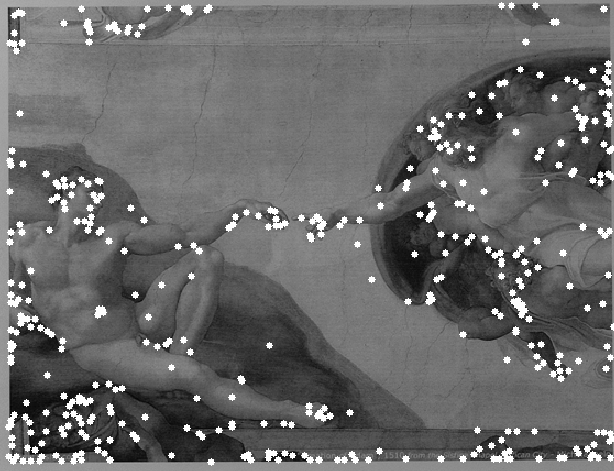
\includegraphics[width=0.8\textwidth]{SIFT}
        \captionof{figure}{Méthode SIFT sur \textit{La création d'Adam}, l'\oe{}uvre de Michel-Ange}
        \label{fig:sift}
    \end{minipage}
    \\\\

    \item \textit{Calcul de la similarité entre les deux images. Le principe est de considérer pour un pixel p1 de l’image 1, une fenêtre rectangulaire centrée en p1 et de calculer sa corrélation (sa distance) avec une fenêtre dans la deuxième image. La fonction de corrélation est alors maximum (distance minimum) en p2 correspondant à p1 dans la deuxième image. \\}
    
    \textit{Le travail consistera donc à :}
    
    \begin{enumerate}
        \item  \textit{Calculez pour chaque point d’intérêt de l’image gauche sa similarité, avec une des fonctions ci-dessus, avec chacun des points de l’image droite. On affichera le meilleur point correspondant et son score. Un ensemble de pré-traitements sera très certainement nécessaire pour éviter de tester tous les points entre eux.}
        \\
        
        Pour calculer la similarité entre deux images, j'ai procédé de la façon suivante : \\
        
        \begin{enumerate}
            \item Après avoir choisi une fonction de calcul de points d'intérêts (en l'occurrence la méthode \verb+SIFT+), j'applique une fonction de floutage (\verb+cv2.blur+) sur chacune des images afin de lisser les différences.\\
        
            \item Pour chaque point d'intérêt de chaque image, je fais une fenêtre de taille prédéterminée autour du point grâce à la méthode \verb+window_around+.\\
            
            \item Pour chaque fenêtre de chaque point d'intérêt, je calcule le coût (fonction de similarité). Si ce coût est inférieur à tous les coûts des fenêtres précédentes, le point d'intérêt associé est mémorisé. Le dernier point d'intérêt à être mémorisé est le meilleur (meilleure similarité entre les deux images). La fonction de coût est calculée grâce à la méthode \verb+cost+.
            
            \item Enfin, la méthode \verb+plot_windows+ est appelée pour afficher la meilleure fenêtre. Dans le cas de la figure~\ref{fig:similaritiesSAD},  \verb+plot_windows+ est appelée lorsque le coût est en dessous d'un certain seuil, ce qui permet d'afficher plusieurs points d'intérêt.
            \\\\
            

            

        \centerline{\begin{minipage}{1.3\linewidth}
            \centering
            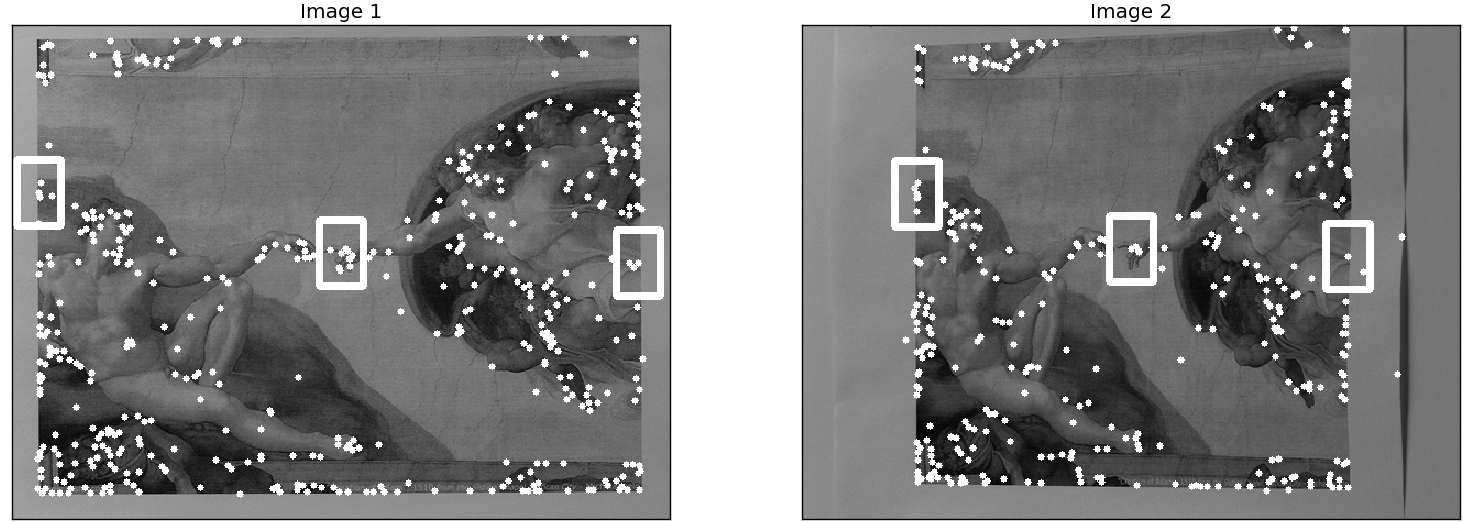
\includegraphics[width=1.1\textwidth]{similaritiesSAD}
            \captionof{figure}{Similarités entre \textit{La création d'Adam} originale et une version avec rotation de 45°. Paramètres : \textit{SAD}, \textit{SIFT}.}
            \label{fig:similaritiesSAD}
        \end{minipage}}
        
        \vspace{5mm}
        Pour la figure~\ref{fig:similaritiesSSD}, j'ai choisi d'utiliser une fonction \textit{SSD}. Le maximum de similarité est atteint pour le point entouré par l'unique fenêtre. Pour ce point, le coût atteint une valeur de 102761.
        \\
    
        \centerline{\begin{minipage}{1.3\linewidth}
            \centering
            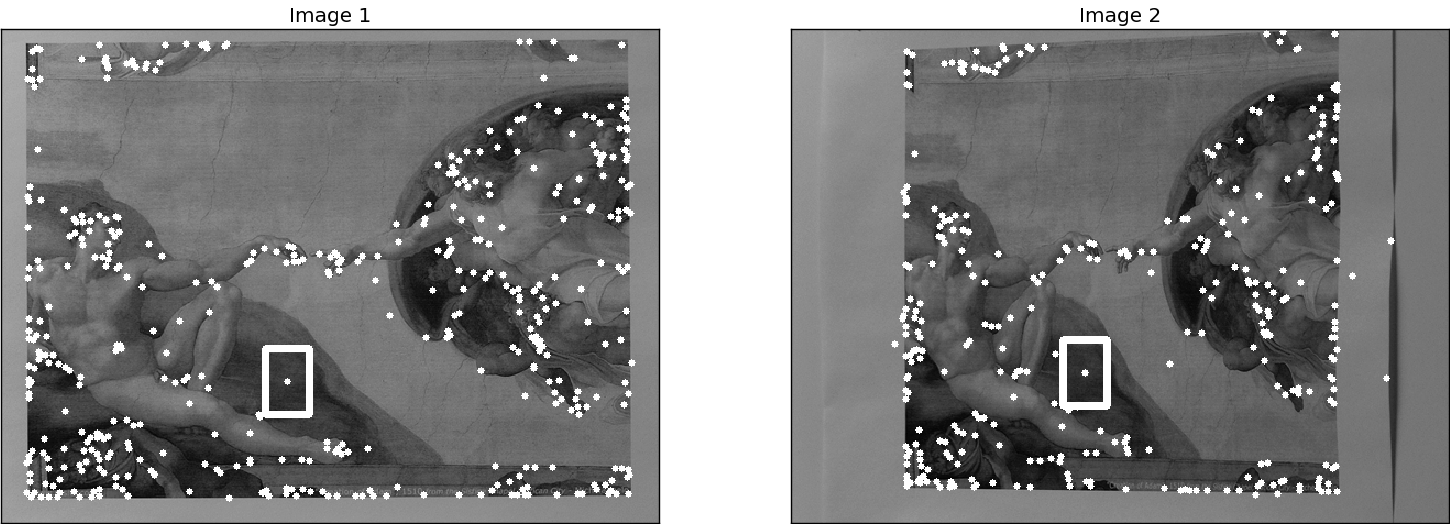
\includegraphics[width=1.1\textwidth]{similaritiesSSD}
            \captionof{figure}{Similarités entre \textit{La création d'Adam} originale et une version avec rotation de 45°. Paramètres : \textit{SSD}, \textit{SIFT}.}
            \label{fig:similaritiesSSD}
        \end{minipage}}

            \end{enumerate}
  
        \item  \textit{Faire de même mais en échangeant les images de droite et de gauche. Obtient-on le même résultat ? Commentez ces résultats.}
        
        Après avoir échangé les images de gauche et de droite, on observe en figure~\ref{fig:similaritiesSSDinverted} que le point d'intérêt de similarité maximum est identique au précédent. De même, le calcul du coût donne une valeur strictement identique de 102761. 
        
        Pour le coût, le fait que l'on retrouve le même résultat s'explique assez simplement par la symétrie de la fonction de calcul par rapport aux images. Les calculs de points d'intérêt se faisant indépendamment pour les deux images, il est logique que les points résultants soient identiques que l'on prenne les images de gauche à droite ou inversement. \\
        
        \centerline{\begin{minipage}{1.3\linewidth}
            \centering
            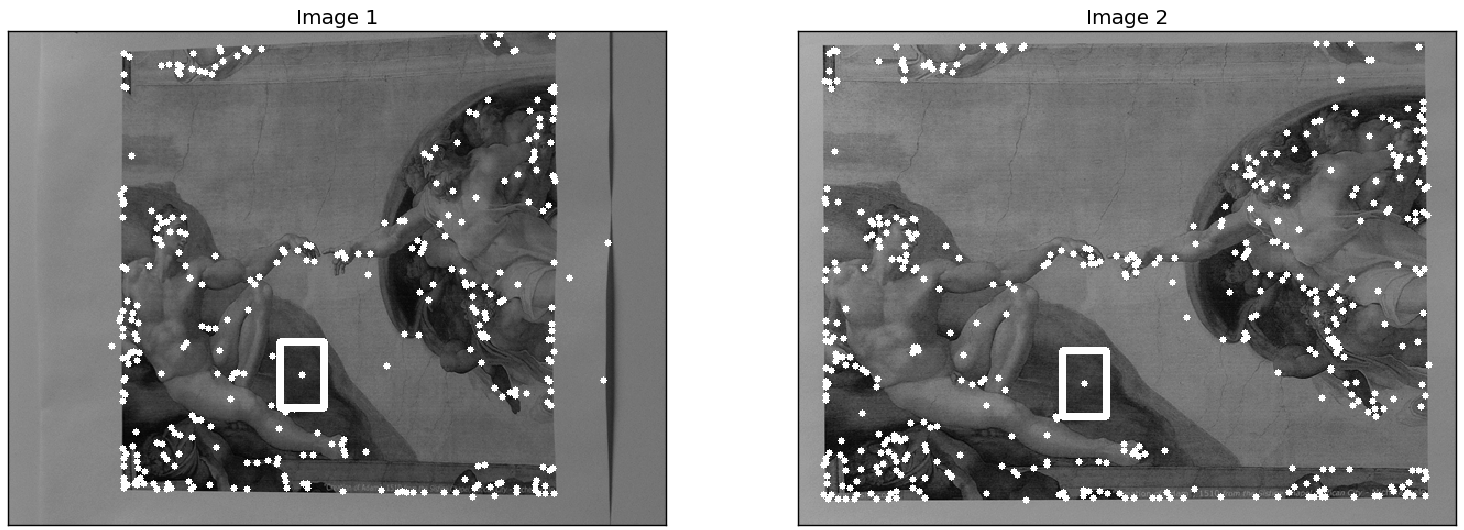
\includegraphics[width=1.1\textwidth]{similaritiesSSDinverted}
            \captionof{figure}{Similarités entre \textit{La création d'Adam} originale et une version avec rotation de 45°. Paramètres : \textit{SSD}, \textit{SIFT}, images inversées.}
            \label{fig:similaritiesSSDinverted}
        \end{minipage}}
        
    \end{enumerate}
    
    \vspace{5mm}
    
    \item Suite à la mise à jour d'OpenCV en version 3.0 puis 3.1 (version utilisée pour ce TP), les méthodes \verb+BFMatcher+ et \verb+FlannBasedMatcher+ ne fonctionnent pas correctement. Les environnements testés sont Ubuntu 14.04 et Max OSX El Capitan. Le seul résultat que j'ai réussi à obtenir est pour la méthode \verb+BFMatcher+ (figure~\ref{fig:bfmatcher}).
    
    Cette méthode donne de bons résultats pour ce type d'images (ce qui n'est pas le cas pour d'autres catégories d'images que j'ai pu tester). Néanmoins, son mode d'action est assez consommateur en ressources : pour chaque descripteur de la première image, la méthode trouve le descripteur le plus proche dans la deuxième image en les essayant tous un par un.
    
    \vspace{5mm}
    
    \centerline{\begin{minipage}{1.3\linewidth}
        \centering
        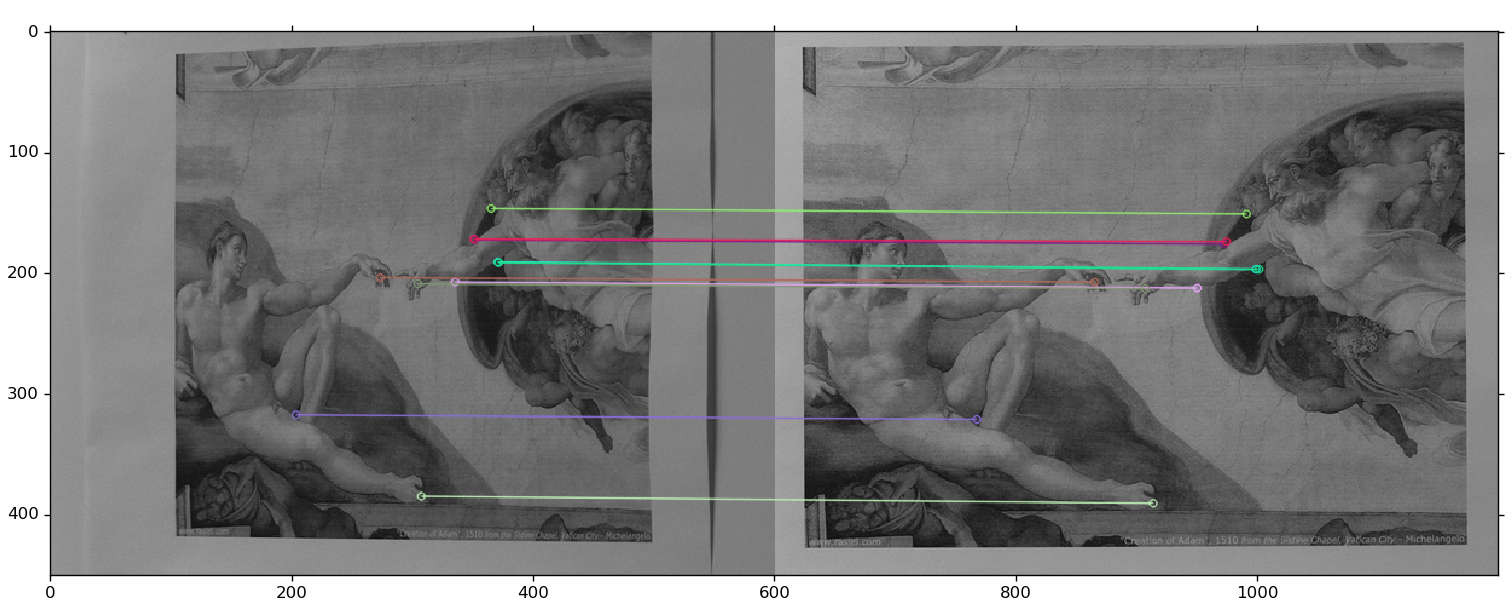
\includegraphics[width=1.1\textwidth]{bfmatcher}
        \captionof{figure}{Application de la méthode \textit{BFMatcher} entre \textit{La création d'Adam} originale\\ et une version avec rotation de 45°.}
        \label{fig:bfmatcher}
    \end{minipage}}
    
\end{enumerate}

\newpage

\section{Implémenter votre propre détecteur de Harris}

\subsection{Structure du détecteur}

    Toutes les méthodes décrites sont situées dans la classe \verb+HomemadeHarris+.

    \subsubsection{Lissage de l'image par l'opérateur de Sobel}
    
        Appelé par la méthode \verb+sobel_transformation+, le lissage de l'image est effectué grâce à la méthode \verb+cv2.Sobel+, afin de garder les gradients selon x et y. Un seuil est nécessaire : par défaut, je l'ai fixé à 5.

    \subsubsection{Calcul de $I_{x}^{2}$, $I_{y}^{2}$ et $I_{xy}$}
    
        En appelant la méthode \verb+gaussian_blur+, on calcule puis on lisse $I_{x}^{2}$, $I_{y}^{2}$ et $I_{xy}$ avec un filtre gaussien. Un paramètre de lissage, \textit{smoothing\_factor}, est nécessaire. Par défaut, celui-ci est de (1, 1).
    
    \subsubsection{Calcul de la fonction de Harris}
    
        Le calcul de la fonction de Harris se fait en appelant la méthode \verb+harris_function+. La méthode renvoie le résultat du calcul. En figure~\ref{fig:harris}, nous pouvons observer la pertinence de ce détecteur pour détecter les contours dans une image. En revanche, les temps de calculs peuvent être longs.
    
        \centerline{\begin{minipage}{1.3\linewidth}
            \centering
            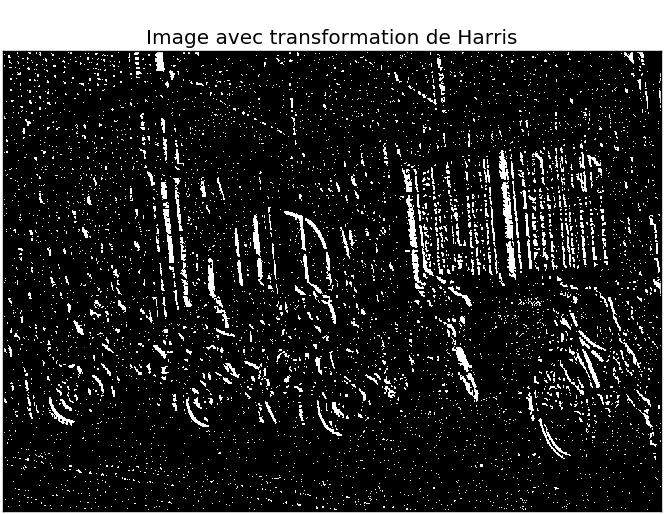
\includegraphics[width=0.6\textwidth]{harris}
            \captionof{figure}{Calcul de la fonction de Harris sur l'image \textit{bike}. \\Paramètres : \textit{window\_size}=10, \textit{seuil\_sobel}=5, \textit{smoothing\_factor}=(1, 1)}
            \label{fig:harris}
        \end{minipage}}
        
    \subsubsection{Extraction des maxima locaux positifs}
        
        Pour extraire les maxima locaux positifs, on définit un voisinage (de 3 par défaut) sur lequel on ne va retenir que le maximum. On trie ensuite parmi ces maxima locaux pour en déduire les \textit{n} maxima globaux de l'image, \textit{n} étant à choisir. Les méthodes \verb+image_improvement+ et \verb+plot+ sont appelées ici.
        
    \vspace{10mm}
    
    Une fois ces étapes effectuées, on obtient la figure~\ref{fig:harris_filtered}. Malgré un bruit de fond assez présent (assez facilement supprimable par ailleurs), la qualité du détecteur semble correcte. Comme pistes d'améliorations, on peut citer l'utilisation de filtres médians contre le bruit par exemple. 
    
    \vspace{5mm}
        
    \centerline{\begin{minipage}{1.3\linewidth}
        \centering
        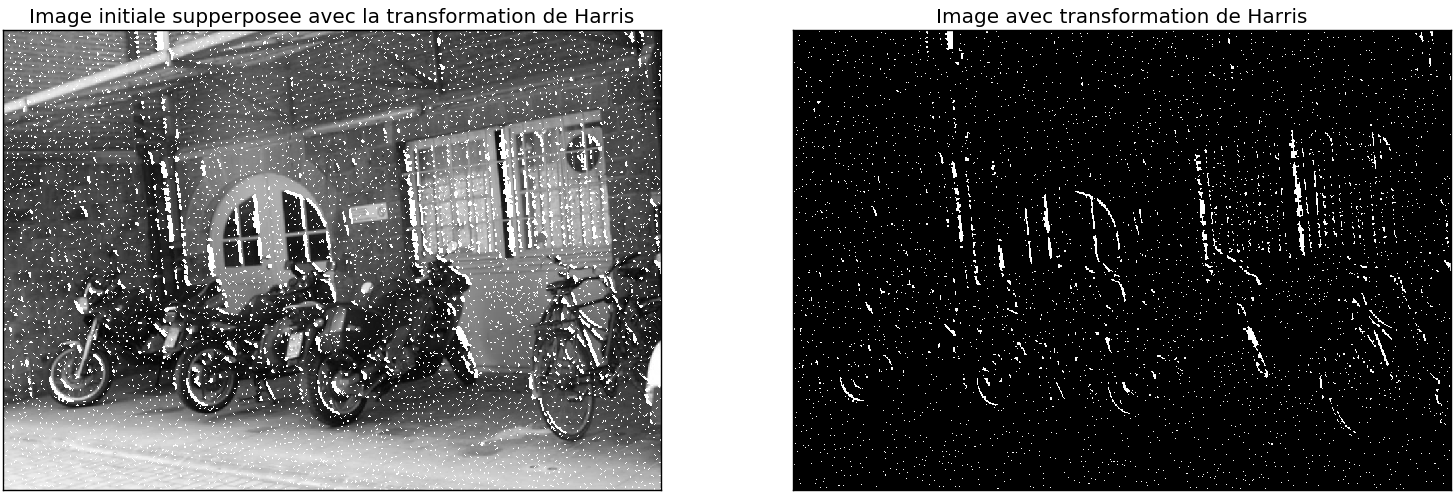
\includegraphics[width=\textwidth]{harris_filtered}
        \captionof{figure}{Calcul de la fonction de Harris sur l'image \textit{bike}. \\Paramètres : \textit{window\_size}=10, \textit{seuil\_sobel}=5, \textit{smoothing\_factor}=(3, 3), \textit{nb\_best\_points}=100000}
        \label{fig:harris_filtered}
    \end{minipage}}
\end{document}